\documentclass[32pt]{article}

\usepackage[utf8]{inputenc}
\usepackage[a4paper]{geometry}

\usepackage{amsfonts}
\usepackage{amsmath}
\usepackage{ccicons}
\usepackage{color}
\usepackage{listings}
\usepackage{tikz}
\usepackage{hyperref}

\lstloadlanguages{C++}
    \lstset{%
        language={C++},
        basicstyle=\ttfamily,
        keywordstyle=\color{blue},
        showstringspaces=false,
        escapechar={§},
        escapeinside={(*@}{@*)}
    }

\lstdefinestyle{cpp20}{language={C++},
  morekeywords={noexcept,co_await,co_return,co_yield,requires,consteval,constinit,concept}
}

\tikzstyle{every picture}+=[remember picture]

\definecolor{co_return_object}{RGB}{179,179,255}
\definecolor{co_promise}{RGB}{255,179,179}
\definecolor{co_awaitable}{RGB}{179,255,179}


\title{C++20 Coroutines - Cheat Sheet}
\author{Andreas Weis}

\pagenumbering{gobble} 

\newif\ifnocolors
% \nocolorstrue
 \nocolorsfalse


\begin{document}
  \ifnocolors
  \begin{lstlisting}[style=cpp20,numbers=left]
struct ReturnType / std::coroutine_traits<ReturnType, ...> { 
  struct promise_type {
    promise_type(T...);  // opt.
    ReturnType get_return_object();
    std::suspend_always initial_suspend();
    // ---- (*@$\Uparrow$@*) Start / (*@$\Downarrow$@*) Shutdown ----
    void return_value(T); / void return_void();
    void unhandled_exception();
    std::suspend_always final_suspend() noexcept;
\end{lstlisting}\begin{lstlisting}[style=cpp20]
  };
};
  \end{lstlisting}

  \begin{lstlisting}[style=cpp20,numbers=left]
struct Awaitable {
  bool await_ready();
  void await_suspend(std::coroutine_handle<promise_type>);
  void await_resume(); 
};
\end{lstlisting}

  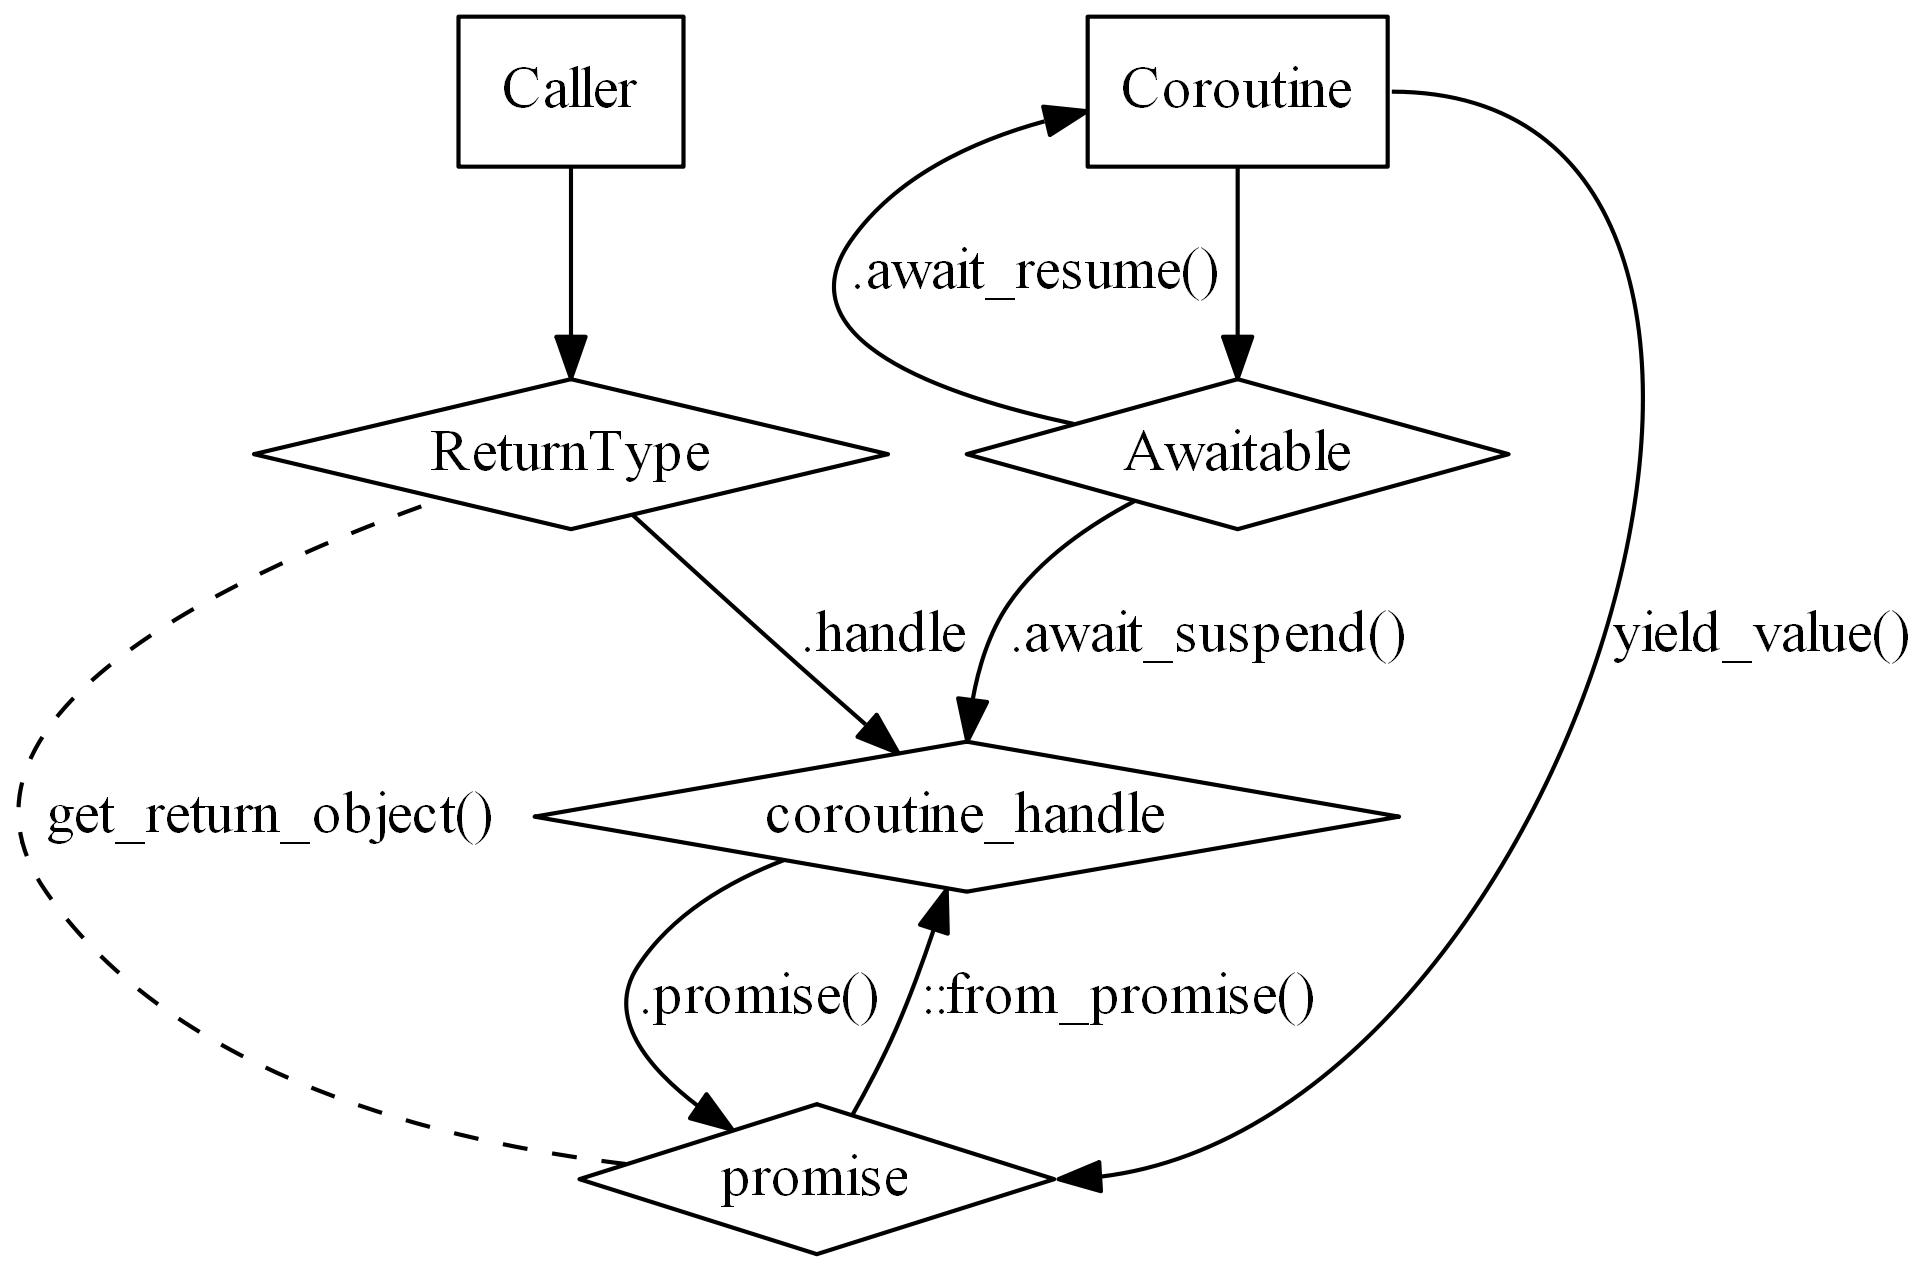
\includegraphics[height=.5\textheight]{gfx/figure_bw.png}
  
  \else

  \begin{lstlisting}[style=cpp20,numbers=left]
struct (*@\tikz[baseline,inner sep=0]\node[anchor=base](ar100){};@*)ReturnType(*@\tikz[baseline,inner sep=0]\node[anchor=base](br100){};@*) / std::coroutine_traits<(*@\tikz[baseline,inner sep=0]\node[anchor=base](mr100){};@*)ReturnType(*@\tikz[baseline,inner sep=0]\node[anchor=base](nr100){};@*), ...> { 
  struct (*@\tikz[baseline,inner sep=0]\node[anchor=base](cr100){};@*)promise_type(*@\tikz[baseline,inner sep=0]\node[anchor=base](dr100){};@*) {
    (*@\tikz[baseline,inner sep=0]\node[anchor=base](kr100){};@*)promise_type(T...);(*@\tikz[baseline,inner sep=0]\node[anchor=base](lr100){};@*)  // opt.
    (*@\tikz[baseline,inner sep=0]\node[anchor=base](er100){};@*)ReturnType(*@\tikz[baseline,inner sep=0]\node[anchor=base](fr100){};@*) get_return_object();
    (*@\tikz[baseline,inner sep=0]\node[anchor=base](gr100){};@*)std::suspend_always(*@\tikz[baseline,inner sep=0]\node[anchor=base](hr100){};@*) initial_suspend();
    // ---- (*@$\Uparrow$@*) Start / (*@$\Downarrow$@*) Shutdown ----
    void return_value(T); / void return_void();
    void unhandled_exception();
    (*@\tikz[baseline,inner sep=0]\node[anchor=base](ir100){};@*)std::suspend_always(*@\tikz[baseline,inner sep=0]\node[anchor=base](jr100){};@*) final_suspend() noexcept;
\end{lstlisting}\begin{lstlisting}[style=cpp20]
  };
};
  \end{lstlisting}
  
  \tikz[overlay]\filldraw[blue, opacity=0.3] ([shift={(0,-0.5ex)}]ar100) rectangle ([shift={(0,2ex)}]br100);
  \tikz[overlay]\filldraw[blue, opacity=0.3] ([shift={(0,-0.5ex)}]mr100) rectangle ([shift={(0,2ex)}]nr100);
  \tikz[overlay]\filldraw[red, opacity=0.3] ([shift={(0,-0.5ex)}]cr100) rectangle ([shift={(0,2ex)}]dr100);
  %\tikz[overlay]\filldraw[red, opacity=0.3] ([shift={(0,-0.5ex)}]kr100) rectangle ([shift={(0,2ex)}]lr100);
  \tikz[overlay]\filldraw[blue, opacity=0.3] ([shift={(0,-0.5ex)}]er100) rectangle ([shift={(0,2ex)}]fr100);
  \tikz[overlay]\filldraw[green, opacity=0.3] ([shift={(0,-0.5ex)}]gr100) rectangle ([shift={(0,2ex)}]hr100);
  \tikz[overlay]\filldraw[green, opacity=0.3] ([shift={(0,-0.5ex)}]ir100) rectangle ([shift={(0,2ex)}]jr100);



  \begin{lstlisting}[style=cpp20,numbers=left]
struct (*@\tikz[baseline,inner sep=0]\node[anchor=base](ar101){};@*)Awaitable(*@\tikz[baseline,inner sep=0]\node[anchor=base](br101){};@*) {
  bool await_ready();
  void await_suspend(std::coroutine_handle<(*@\tikz[baseline,inner sep=0]\node[anchor=base](cr101){};@*)promise_type(*@\tikz[baseline,inner sep=0]\node[anchor=base](dr101){};@*)>);
  void await_resume(); 
};
\end{lstlisting}
  
  \tikz[overlay]\filldraw[green, opacity=0.3] ([shift={(0,-0.5ex)}]ar101) rectangle ([shift={(0,2ex)}]br101);
  \tikz[overlay]\filldraw[red, opacity=0.3] ([shift={(0,-0.5ex)}]cr101) rectangle ([shift={(0,2ex)}]dr101);

  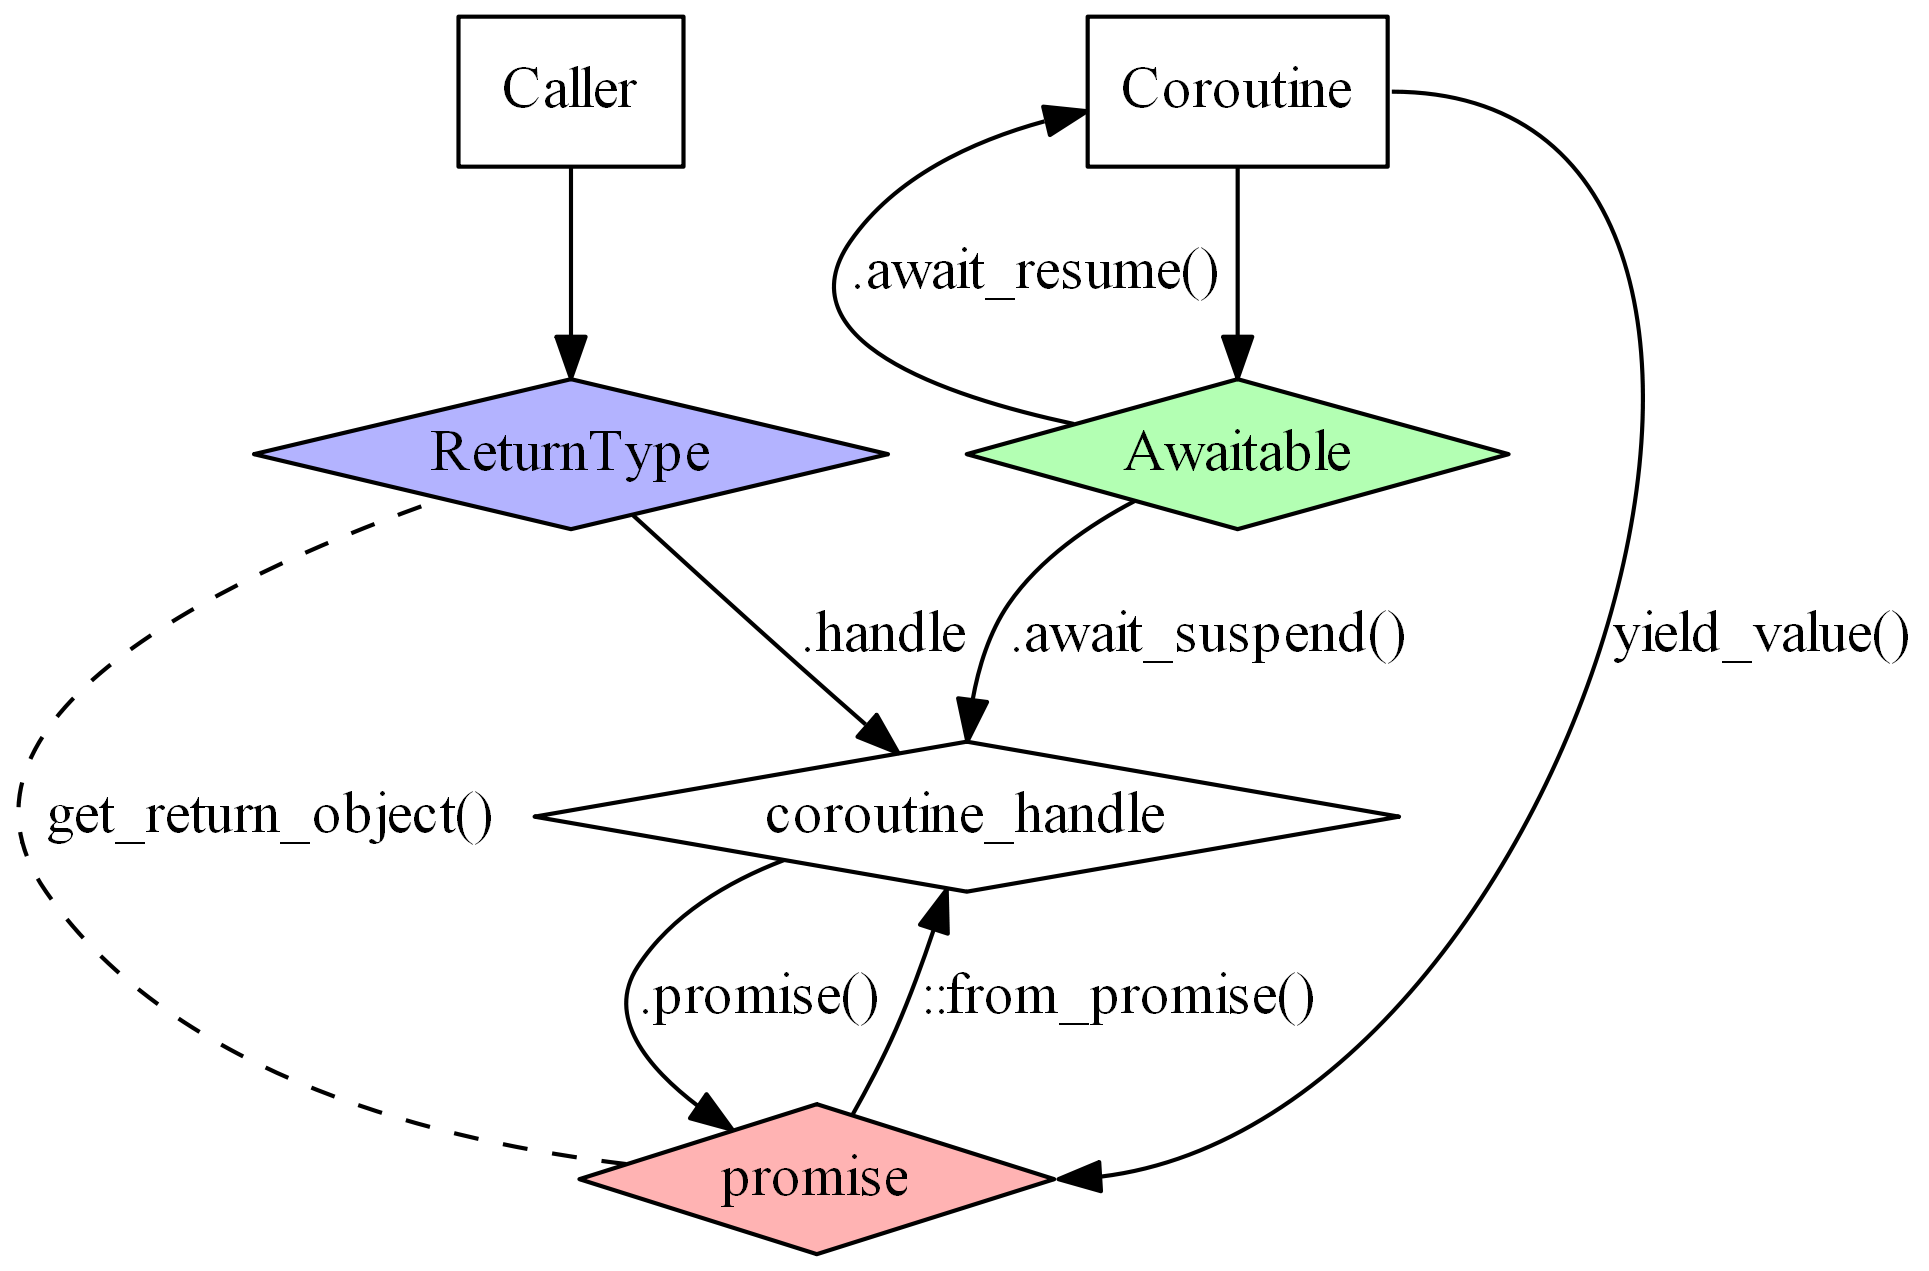
\includegraphics[height=.5\textheight]{gfx/figure.png}
  
  \fi
  
  \vspace{1em}
  
  \begin{flushright}
    \ccby \tiny{Andreas Weis - C++ 20 Coroutine Cheat Sheet}
  \end{flushright}
\end{document}
